\chapter{Lip Reed}\label{ch:lipreed}
Brass instruments are excited by the lips of the player. The opening and closing of the lips causes a vibration

Sections \ref{sec:webstersExcitation} and \ref{sec:pulseTrain} presented a physically inspired pulse train that attempts to model this opening and closing of the lips using a clipped sinusoidal signal. A more physical approach, that is bidirectional, is to model a lip as a mass-spring system that interacts with the left boundary of the tube.
Lip reed model



Coupling to Tube

The authors of \cite{Fletcher1998} state that all wind-instrument reeds fall into one of three categories: the single reed, (clarinet, saxophone), the double reed (oboe, bassoon) and the lip reed (trumpet, trombone). 

And recent work includes vortex-induced vibration [\hyperref[ch:listOfPublications]{S1}] 

The literature describes lip reed models with varying degrees of freedom (DoF)
In this work, the lip reed will be modelled as a single one-DoF mass-spring-damper system. This model is used to simulate the lip reed in paper \citeP[H] where an additional collision has been added. This chapter presents the lip reed without the collision, but will be elaborated on in Chapter \ref{ch:trombone}. \todo{check} The bulk of this chapter follows \cite{Harrison2018}. 

Lip reed will be coupled to the first-order system of equations presented in \ref{sec:firstOrderSystem} 



\section{Mass-spring systems revisited: Damping}\label{sec:massSpringDamping}
Before moving on to the lip reed system, a small extension to the mass-spring system given in Section \ref{sec:massSpringSystem} will be given here. 

Recall the mass spring system presented in Eq. \eqref{eq:massSpringPDE}, where $u=u(t)$ is the displacement of the mass from its equilibrium position.Damping can be easily be added to yield a mass-spring-damper system: 
\begin{equation}\label{eq:massSpringDampingPDE}
    M\ddot u = -Ku - R\dot u,
\end{equation}
with mass $M$ (in kg), spring constant $K$ (N/m) and damping coefficient $R$ (in kg/s). Figure \ref{fig:massSpringDamper} shows the behaviour of the system for different values of $R$. 

\def\figWidth{0.32}
\begin{figure}[b]
    \centering
    \subfloat[$R=0$.\label{fig:massSpringDamper1}]{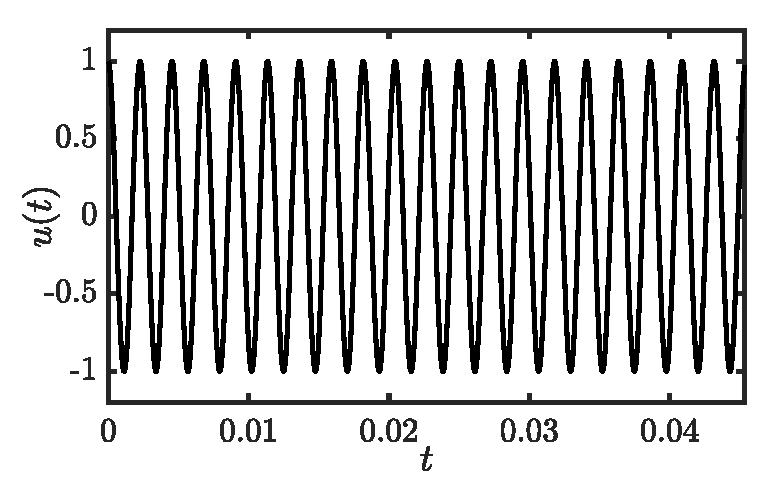
\includegraphics[width=\figWidth\textwidth]{figures/exciters/lipreed/massSpringDamper1.eps}}\hfill
    \subfloat[$R=50$.\label{fig:massSpringDamper2}]{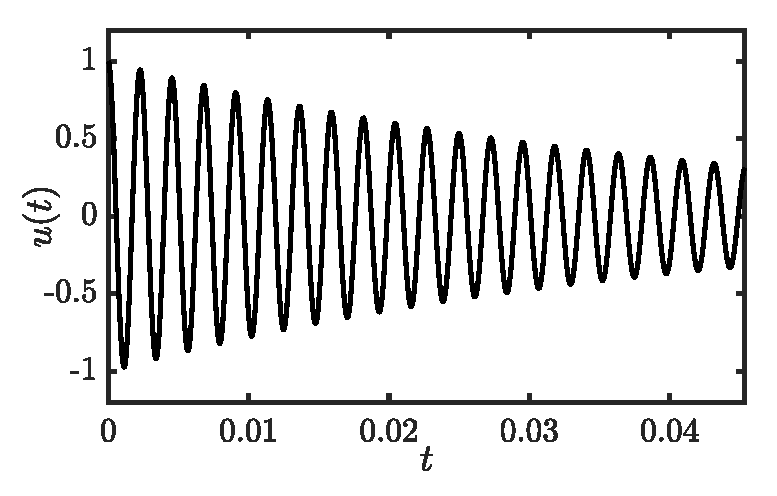
\includegraphics[width=\figWidth\textwidth]{figures/exciters/lipreed/massSpringDamper2.eps}}\hfill
    \subfloat[$R=200$.\label{fig:massSpringDamper3}]{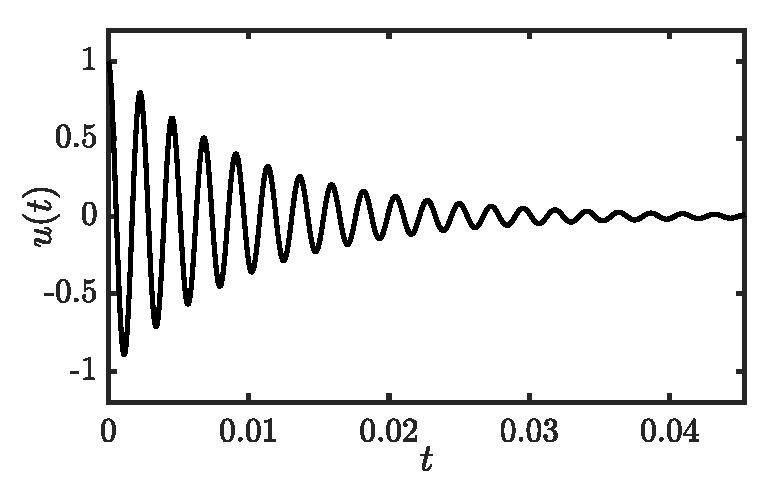
\includegraphics[width=\figWidth\textwidth]{figures/exciters/lipreed/massSpringDamper3.eps}}
    \caption{The mass-spring-damper system in Eq. \eqref{eq:massSpringDampingPDE} for different values of $R$. \label{fig:massSpringDamper}}
\end{figure}

Equation \eqref{eq:massSpringDampingPDE} can then be discretised to the following FD scheme:
\begin{equation}\label{eq:massSpringDampingFDS}
    M\dtt \un = -K\un - R\dtd \un.
\end{equation}
Expanding and solving for $u^{n+1}$ yields the following update equation (before division with the term multiplied onto $u^{n+1}$):
\begin{equation}\label{eq:massSpringDampingUpdate}
    \left(1+\frac{Rk}{2M}\right)u^{n+1} = 2 \un - u^{n-1} - \frac{Kk^2}{M}\un + \frac{Rk}{2M}u^{n-1}.
\end{equation}

\subsection{Energy analysis}
Following Section \ref{sec:energyAnalysis} (without explicitly following the steps for brevity), one can obtain the energy of Eq. \eqref{eq:massSpringDampingFDS} through a multiplication of the scheme by $(\dtd \un)$ to get
\begin{equation}\label{eq:massSpringDampingPreEnergyBalance}
    M(\dtt \un)(\dtd \un) = -K(\dtd \un)\un - R(\dtd \un)^2.
\end{equation}
As there is damping present in the system, the energy balance will be of the form 
\begin{equation*}
    \dtp \h = -\q.
\end{equation*}
Using identities \eqref{eq:prodIdentity1} and \eqref{eq:prodIdentity2}, $\h$ and $\q$ can be obtained from Eq. \eqref{eq:massSpringDampingPreEnergyBalance} 
\begin{equation}\label{eq:energyBalanceMassSpringDamper}
    \h = \t + \v, \qwiq
    \t = \frac{M}{2}(\dtm\un)^2, \qaq \v = \frac{K}{2}\un e_{t-}\un.
\end{equation} 
and
\begin{equation}\label{eq:massDampingEnergy}
    \q = R(\dtd \un)^2.
\end{equation}

Figure \ref{fig:massSpringDamperEnergy} shows the energy output of the mass spring damper system with $R = 50$ and $f_0 = 2\pi\sqrt{K/M} = 440$ Hz. One can observe that the damping term causes the system to lose energy when the mass is in motion (high kinetic energy).
\begin{figure}[h]
    \centering
    \begin{tikzpicture}[->,node distance=3cm,
        thick,main node/.style={circle,draw}]
    
        \node[] (image) at (0,0) {
        \includegraphics[width=\textwidth]{figures/exciters/lipreed/massSpringDamperEnergy.eps}
        };
    
        \node[] (he) at (0.2,0.5) {\small $\mathfrak{h}_\text{e}$};

        \node[] (h) at (-5.8, 1) {\small $\mathfrak{h}$};
        \node[] (v) at (-5.8, 0.5) {\small $\color{red}\mathfrak{v}$};
        \node[] (t) at (-5.8, 0) {\small $\color{blue}\mathfrak{t}$};
      \end{tikzpicture}
      \caption{The potential (red), kinetic (blue), and total (black) energy of the mass-spring-damper system. The right panel shows the normalised energy (according to Eq. \eqref{eq:normalisedEnergyDamping}) and shows that the deviation of the energy is within machine precision. \label{fig:massSpringDamperEnergy}}
\end{figure}

\section{Continuous time}\label{sec:lipreedContinuous}
As mentioned at the beginning of this chapter, the lip reed will be modelled as a mass-spring-damper system as in Eq. \eqref{eq:massSpringDampingPDE}. The system will be coupled to an acoustic tube described by the first-order system of PDEs described in Section \ref{sec:firstOrderSystem}, Eq. \eqref{eq:firstOrderSystem}.
% :
% \begin{subequations}\label{eq:firstOrderSystemLipReedCh}
%     \begin{align}
%         \frac{S}{\rho_0 c^2}\partial_t p &= -\partial_x(Sv),\label{eq:contPressureLipReedCh}\\
%         \rho_0\partial_tv &= -\partial_xp\label{eq:discVelocityLipReedCh},
%     \end{align}
% \end{subequations} %An additional term  due to the pressure difference between the mouth and the tube is added to the equation and t

Using dots to denote derivatives with respect to time $t$, the PDE of the lip reed connected to an acoustic tube is defined as
\begin{equation}
    M_\text{r}\ddot y = -K y - R \dot y + S_\text{r}\Delta p.
\end{equation}
with displacement of the lip reed from equilibrium $y = y(t)$ (in m), mass of the lip reed $M_\text{r} > 0$ (in kg), lip stiffness $K\geq 0$ (in N/m), damping coefficient $R\geq 0$ (in kg/s), effective surface area of the lip $S_\text{r}\geq 0$ (in m$^2$). Furthermore,  
\begin{equation}\label{eq:deltaP}
    \Delta p = \Delta p(t) = P_\text{m} - p(0,t)
\end{equation}
is the difference between the pressure in the mouth $P_\text{m} = P_\text{m}(t)$ and the pressure at the left boundary of the acoustic tube $p(0,t)$ (all in Pa). The acoustic tube can be described by the first-order system presented in Section \ref{sec:firstOrderSystem}.
To reduce the number of variables in later derivations in this chapter, one can perform the following change of variables
\begin{equation}
    \ddot y = -\omega_0^2 y - \sigma_\text{r} \dot y + \frac{S_\text{r}}{M_\rtxt}\Delta p,
\end{equation}
with angular frequency of the lip reed $\omega_0 = \sqrt{K/M_\text{r}}$ (rad/s) and loss parameter $\sigma_\text{r} = R / M_\text{r}$ (s$^{-1}$). 
\begin{figure}[ht]
    \centering
    \begin{tikzpicture}
    
    \def\radius{6}; % Radius of the string (>2!)
    \pgfmathsetmacro{\reps}{3}; % How may back-and-forths in the drawing of the springs
    \def\bowSpacing{0.2};
    \def\drawingSpacing{1.5}
    \def\bowWidth{5};
    
    \def\woodWidth{1}; %>0.3
    \def\massWidth{2};
    \def\bridgeHeight{3};
    \def\bridgeWidth{4};
    \def\cornerRadius{0.15};
    \def\stringWidth{0.2};
    \pgfmathsetmacro{\tinyRadius}{\stringWidth*0.1};
    \pgfmathsetmacro{\stringWidthMinTinyRad}{((\stringWidth-(2*\tinyRadius)))*0.5};
    
    % draw airflow
    
    %draw airflow
    \def\rightAirFlow{0}; % have the right airflow bulge (1) or not (0)
    \foreach \idx in {1,...,5}
    {
        \pgfmathsetmacro{\scaleLeft}{0.5 - 0.1 * \idx};
        \ifnum\rightAirFlow=1
            \pgfmathsetmacro{\scaleRight}{0.5 - 0.1 * \idx};
        \else
            \pgfmathsetmacro{\scaleRight}{0};
        \fi
        \begin{scope}[decoration={
            markings,
            mark=between positions 0.15 and 0.85 step 0.35
         with {\arrow{>}}}
            ]
        % \node at (0, \idx) {\scale};
         \draw [gray!40, 
         xshift=-2.5cm, 
         yshift= -\idx * 0.3cm, 
         dotted, 
         line width=0.3mm, postaction={decorate}] plot [smooth, tension = 0.5] coordinates { (0,1*\scaleLeft) (1,0.75*\scaleLeft) (2,0) (4, 0) (5, 0.75*\scaleRight) (6,1*\scaleRight)} ;
         \end{scope}
    }
    % \def\scale{0.5};
    % \draw [gray, xshift=-2.5cm, yshift=-0cm] plot [smooth, tension = 0.5] coordinates { (0,1*\scale) (1,0.75*\scale) (2,0) (4, 0) (5, 0.75*\scale) (6,1*\scale)};
    % \def\scale{0.25};
    % \draw [gray, xshift=-2.5cm, yshift=-1.2cm] plot [smooth, tension = 0.5] coordinates { (0,1*\scale) (1,0.75*\scale) (2,0) (4, 0) (5, 0.75*\scale) (6,1*\scale)};
    % \def\scale{0};
    % \draw [gray, xshift=-2.5cm, yshift=-1.5cm] plot [smooth, tension = 0.5] coordinates { (0,1*\scale) (1,0.75*\scale) (2,0) (4, 0) (5, 0.75*\scale) (6,1*\scale)};
    
    \node (r0) at ( 1.0,  -0.5 ) {}; % root
    \node (s0) at ( 1.0, 0.1 ) {}; % extreme
    \node (s1) at ( 1.6, 0.1 ) {}; % extreme

    % DRAW TREE
    \fill[fill=white] (r0.center)--(s0.center)--(s1.center);
    
    % \draw plot [smooth] coordinates {(-3, -3) (-2, 2) (-1, -3};
    \node at (0,0) [rectangle,draw, fill = white, minimum height=1cm,minimum width= \massWidth cm] (Mr) {$M_\text{r}$};
    %top
    % \draw[-] (-3, 2) -- (3, 2) node[below, midway] (top) {};
    % \draw[-] (-2, 3) -- (4, 3) node[below, midway] (top) {};
    % \draw[-] (-3, 2) -- (-2, 3) node[below, midway] (top) {};
    % \draw[-] (4, 3) -- (3, 2) node[below, midway] (top) {};
    \draw[-] (-2.5, 2.5) -- (3.5, 2.5) node[below, midway] (top) {};
    %bottom
    \draw[-] (-3, -2) -- (3, -2) node[below, midway] (bottom) {};
    \draw[-] (-2, -1) -- (4, -1) node[below, midway] (bottom) {};
    \draw[-] (-3, -2) -- (-2, -1) node[below, midway] (top) {};
    \draw[-] (4, -1) -- (3, -2) node[below, midway] (top) {};

    % draw mass
    
    \draw[-] (-1, 0.5) -- (0, 1.5) node[] (left) {};

    \draw[-] (1, 0.5) -- (2, 1.5) node[] (topRight) {};

    \draw[-] (0, 1.5) -- (2, 1.5) node[] (top) {};

    \draw[-] (2, 1.5) -- (2, 0.5) node[] (right) {};

    \draw[-] (0.5 * \massWidth, -0.5) -- (2, 0.5) node[] (bottomRight) {};

    \node[rotate = 0] at (0.5, 1) (Sr) {$S_\text{r}$};

    \def\xOffset{0.3};
    % draw spring
    \filldraw[black] (-0.5 + \xOffset, 2.5) circle (1pt) node[anchor=center](topSpring){};    
    \draw[-] (-0.5 + \xOffset, 2.5) -- (-0.5 + \xOffset, 2.3);
    \draw[-] (-0.5 + \xOffset, 2.3) -- (-0.75 + \xOffset, 2.2);
    %switched these around because of the color
    \draw[-] (-0.25 + \xOffset, 2.02) -- (-0.75 + \xOffset, 1.84);
    \draw[-] (-0.75 + \xOffset, 2.2) -- (-0.25 + \xOffset, 2.02);
    \draw[-] (-0.75 + \xOffset, 1.84) -- (-0.25 + \xOffset, 1.66);
    \draw[-] (-0.25 + \xOffset, 1.66) -- (-0.75 + \xOffset, 1.52);
    \draw[-] (-0.75 + \xOffset, 1.52) -- (-0.25 + \xOffset, 1.3);
    \draw[-] (-0.25 + \xOffset, 1.3) -- (-0.5 + \xOffset, 1.2);
    \draw[-] (-0.5 + \xOffset, 1.2) -- (-0.5 + \xOffset, 1.0);
    \filldraw[black] (-0.5 + \xOffset, 1.0) circle (1pt) node[anchor=center](bottomSpring){};    
    \node at (-1 + \xOffset, 1.75) (K) {$K$};
    
    \def\dashpotHeight{-0.25}
    % draw dashpot
    \filldraw[black] (1.5 - \xOffset, 2.5) circle (1pt) node[anchor=center](topDashPot){};
    \draw[-] (1.5 - \xOffset, 2.5) -- (1.5 - \xOffset, 1.4 - \dashpotHeight);

    \draw[-] (1.3 - \xOffset, 1.4 - \dashpotHeight) -- (1.7 - \xOffset, 1.4 - \dashpotHeight);

    \draw[-] (1.25 - \xOffset, 1.7 - \dashpotHeight) -- (1.25 - \xOffset, 1.35 - \dashpotHeight);
    \draw[-] (1.75 - \xOffset, 1.35 - \dashpotHeight) -- (1.75 - \xOffset, 1.7 - \dashpotHeight);

    \draw[-] (1.25 - \xOffset, 1.35 - \dashpotHeight) -- (1.75 - \xOffset, 1.35 - \dashpotHeight);
    \draw[-] (1.5 - \xOffset, 1.35 - \dashpotHeight) -- (1.5 - \xOffset, 1.0);

    \filldraw[black] (1.5 - \xOffset, 1.0) circle (1pt) node[anchor=center](bottomDashpot){};    
    \node at (1.0 - \xOffset, 1.75) (sigma) {$R$};
    
    
    % pressure labels
    \def\pressOffset{0.3}
    \def\backgroundOpacity{0.4}
    \node[fill = white, fill opacity=\backgroundOpacity, text opacity = 1] at (-2, -0.6 - \pressOffset) (Pm) {$P_\text{m}$};
    \node[fill = white, fill opacity=\backgroundOpacity, text opacity = 1] at (0.5, -0.8 - \pressOffset) (deltaP) {$\Delta p$};
    \node[fill = white, fill opacity=\backgroundOpacity, text opacity = 1] at (3.2, -0.6 - \pressOffset) (p) {$p(0,t)$};

    
    % y and H0
    \def\axisLineWidth{0.07};
    \draw[dashed, color = gray] (3.65, 0) -- (1.5, 0);
    \node at (4, 1.5) {$y$};
    
    \draw[->] (3.75, -1.5) -- (3.75, 1.5);
    \node at (4, 0) {$0$};
    \draw (3.75 - \axisLineWidth, 0) -- (3.75 + \axisLineWidth, 0) {};

    \draw (3.75 - \axisLineWidth, -1.5) -- (3.75 + \axisLineWidth, -1.5) {};
    \node at (4.2, -1.5) {$-H_0$};
    
    % width
    \draw[black!70] (-1, 0.6) -- (1, 0.6) {};
    \draw[black!70] (-1, 0.55) -- (-1, 0.65) {};
    \draw[black!70] (1, 0.55) -- (1, 0.65) {};
    \node at (0, 0.75) (w) {$w$};
% \begin{scope}[very thick,decoration={
%     markings,
%     mark=at position 0.5 with {\arrow{>}}}
%     ] 
%     \draw[postaction={decorate}] (-4,0)--(4,0);
% \end{scope}
    
    \end{tikzpicture}
    \caption{Lip-reed system with parameters as appears in Section \ref{sec:lipreedContinuous}. (Adapted from paper \citeP[H].)}
    \label{fig:lipSystem}
\end{figure}

The pressure difference in Eq. \eqref{eq:deltaP} causes a volume flow velocity and follows the Bernoulli equation
\begin{equation}
    U_\text{B} = w[y + H_0]_+\text{sgn}(\Delta p) \sqrt{\frac{2|\Delta p|}{\rho_0}},
\end{equation}
with effective lip-reed width $w$ (in m), density of air $\rho_0$ (in kg/m$^3$), static equilibrium separation $H_0$ (in m) and $[x]_+ = 0.5 (x + |x|)$ describes the `positive part of'. Notice that when $y + H_0 \leq 0$, the lips are closed and the volume velocity $U_\text{B}$ is 0. Another volume flow is generated by the lip reed itself according to
\begin{equation}
    U_\text{r} = S_\text{r} \dot y.
\end{equation}
Assuming that the volume flow velocity is conserved, the total air volume entering the acoustic tube at the left boundary is defined as
\begin{equation}
    S(0)v(0,t) = U_\text{B}(t) + U_\text{r}(t).
\end{equation} 
\section{Discrete time}
\def\nph{}
\def\nphSys{n+1/2}

Following \cite{Harrison2018}, $y$, $\Delta p$, and thereby $U_\text{B}$ and $U_\text{r}$ are placed on the interleaved temporal grid\footnote{Notice that as the lip reed interacts with the boundary of the tube ($x=0$) it is placed on the regular, non-interleaved, spatial grid.}, and the equations presented above can be discretised to the following system:
\begin{subequations}\label{eq:discreteLipSystem}
    \begin{align}
        \delta_{tt}y^{\nphSys} &= -\omega_0^2\mu_{t\cdot}y^{\nphSys}-\sigma_\text{r}\delta_{t\cdot}y^{\nphSys} + \frac{S_\text{r}}{M_\rtxt}\Delta p^{\nphSys},\label{eq:discReed}\\
        \Delta p^{\nphSys} &= P_\text{m} - \mu_{t+}p_0^n,\label{eq:pDiff}\\
        U_\text{B}^{\nphSys} &= w[y^{\nphSys}+H_0]_+\text{sgn}(\Delta p^{\nphSys})\sqrt{\frac{2|\Delta p^{\nphSys}|}{\rho_0}},\label{eq:bernoulli}\\
        U_\text{r}^{\nphSys} &= S_\text{r}\delta_{t\cdot}y^{\nphSys},\label{eq:Ur}\\
        \mu_{x-}(S_{1/2}v_{1/2}^{\nphSys}) &= U_\text{B}^{\nphSys} + U_\text{r}^{\nphSys}.\label{eq:UbUr}
    \end{align}
\end{subequations}
Here, $p_0^n$ and $S_{1/2}v_{1/2}^{\nphSys}$ are discrete values at the left boundary of an acoustic tube described by system \eqref{eq:firstOrderFDS}. Expanding the operators in Eq. \eqref{eq:discReed} and solving for $y^{n+3/2}$ yields
\begin{equation}\label{eq:updateEqLipreed}
    % \left(1 + \frac{\omega_0^2 k^2}{2} + \frac{\sigma_\text{r} k}{2}\right)y^{n+3/2} &= 2 y^{n+1/2} - \left(1 + \frac{\omega_0^2 k^2}{2} - \frac{\sigma_\text{r} k}{2}\right) y^{n-1/2} + \frac{S_\text{r} k^2}{M_\text{r}} \Delta p^{n+1/2}\nonumber\\
    \alpha_\text{r}y^{n+3/2} = 4y^{n+1/2} + \beta_\text{r}y^{n-1/2} + \xi_\text{r}\Delta p^{n+1/2}
\end{equation}
where
\begin{equation}
    \alpha_\text{r} = 2 + \omega_0^2k^2 + \sigma_\text{r} k\ , \quad \beta_\text{r} =  \sigma_\text{r} k - 2 - \omega_0^2 k^2\ , \quad \text{and} \quad \xi_\text{r} = \frac{2 S_\text{r}k^2}{M_\text{r}}.
\end{equation}
Although Eq. \eqref{eq:updateEqLipreed} seems to be implicitly dependent to the pressure difference $\Delta p^{n+1/2}$ it is possible to explicitly solve it. A derivation is shown below.

\subsection{Obtaining $\Delta p$}\label{sec:obtainingDeltaP}
In the following, the superscript $n+1/2$ will be suppressed for $y$, $\Delta p$, $U_\text{B}$, $U_\text{r}$, $S_{1/2}$ and $v_{1/2}$ for brevity. 

Using identities \eqref{eq:identity1} and \eqref{eq:identity4}, Eq. \eqref{eq:discReed} can be rewritten to
\begin{equation*}
    \frac{2}{k} (\delta_{t\cdot} - \delta_{t-})y^{\nph} = -\omega_0^2(k\delta_{t\cdot} + e_{t-})y^{\nph} - \sigma_\text{r}\delta_{t\cdot} y^{\nph} + \frac{S_\text{r}}{M_\text{r}}\Delta p^{\nph},
\end{equation*}
and, after grouping the terms,
\begin{equation}
    a_1\delta_{t\cdot}y^{\nph} - a_2\Delta p^{\nph} - a_3^n = 0,\label{eq:preAEquation}
\end{equation}
where
\begin{equation}\label{eq:aCoeffs}
    a_1 = \frac{2}{k} + \omega_0^2k + \sigma_\text{r} \geq 0, \quad a_2 = \frac{S_\text{r}}{M_\text{r}} \geq 0\ , \quad \text{and} \quad a_3^n = \left(\frac{2}{k} \delta_{t-} - \omega_0^2e_{t-}\right)y^{\nph}\ .
\end{equation}
Note that these conditions can be applied to $a_1$ and $a_2$ as these are calculated solely from non-negative parameters. %The same will be done for other coefficients below.
Equation \eqref{eq:Ur} can then be substituted into Eq. \eqref{eq:preAEquation}
\begin{equation*}
    \frac{a_1}{S_\text{r}}U_\text{r}^{\nph} - a_2 \Delta p^{\nph} - a_3^n = 0,
\end{equation*}
and consequently \eqref{eq:UbUr} to get
\begin{equation}\label{eq:aEquation}
    \frac{a_1}{S_\text{r}}\left(\mu_{x-}(S_{1/2}v_{1/2}^{\nph}) - U_\text{B}^{\nph}\right) - a_2 \Delta p^{\nph} - a_3^n = 0.
\end{equation}
%
Recalling the FD scheme for the pressure of the first-order system in \eqref{eq:discPressure} and evaluating this at $l = 0$ yields
\begin{equation}
    \frac{\bar S_0}{\rho_0 c^2}\delta_{t+}p_0^n = -\delta_{x-}(S_{1/2}v_{1/2}^{\nph}).
\end{equation}
one can obtain get a definition for $\mu_{x-}(S_{1/2}v_{1/2}^{\nph})$, we include the expression for Webster's equation at $l=0$ which, using the following identity (derived from Eq. (2.7d) from \cite{theBible})
\begin{equation}\label{eq:identity}
    \delta_{x\pm} = \pm\frac{2}{h}(\mu_{x\pm} - 1),
\end{equation} 
can be rewritten to
\begin{equation}
    \frac{\bar S_0}{\rho_0 c^2}\delta_{t+}p_0^n = \frac{2}{h} \left(\mu_{x-}(S_{1/2}v_{1/2}^{\nph})-S_{1/2}v_{1/2}^{\nph}\right).
\end{equation}
Then using the same identity \eqref{eq:identity} but for $\delta_{t+}$ we get
\begin{equation}
    \frac{2\bar S_0}{\rho_0 c^2k}(\mu_{t+}p_0^n-p_0^n) = \frac{2}{h} \left(\mu_{x-}(S_{1/2}v_{1/2}^{\nph})-S_{1/2}v_{1/2}^{\nph}\right).
\end{equation}
Using Eq. \eqref{eq:pDiff} we can rewrite this to
\begin{align}
    \frac{\bar S_0h}{\rho_0 c^2k}(P_\text{m} - \Delta p^{\nph}-p_0^n) &= \frac{2}{h} \left(\mu_{x-}(S_{1/2}v_{1/2}^{\nph})-S_{1/2}v_{1/2}^{\nph}\right).\nonumber\\
    \mu_{x-}(S_{1/2}v_{1/2}^{\nph}) &= b_1^n - b_2\Delta p^{\nph}\label{eq:bEquation}
\end{align}
where
\begin{equation}\label{eq:bCoeffs}
    b_1^n = S_{1/2}v_{1/2}^{\nph} + \frac{\bar S_0h}{\rho_0 c^2k} (P_\text{m} - p_0^n), \quad \text{and} \quad b_2 = \frac{\bar S_0h}{\rho_0 c^2k} \geq 0\ .
\end{equation}
We can then substitute Eqs. \eqref{eq:bEquation} and \eqref{eq:bernoulli} into Eq. \eqref{eq:aEquation} to get
\begin{gather}
    \frac{a_1}{S_\text{r}}\left(b_1^n - b_2\Delta p^{\nph} - w[y^{\nph}+H_0]_+\text{sgn}(\Delta p^{\nph})\sqrt{\frac{2|\Delta p^{\nph}|}{\rho_0}}\right) - a_2 \Delta p^{\nph} - a_3^n = 0,\nonumber\\
    - w[y^{\nph}+H_0]_+\text{sgn}(\Delta p^{\nph})\sqrt{\frac{2|\Delta p^{\nph}|}{\rho_0}} - b_2\Delta p^{\nph} - \frac{a_2S_\text{r}}{a_1} \Delta p^{\nph} + b_1^n - \frac{a_3^nS_\text{r}}{a_1} = 0,\nonumber\\
    -c_1^n\text{sgn}(\Delta p^{\nph})\sqrt{|\Delta p^{\nph}|} - c_2\Delta p^{\nph} + c_3^n = 0\label{eq:cEquation}
\end{gather}
where
\begin{equation}\label{eq:cCoeffs}
    c_1^n = w[y^{\nph} + H_0]_+\sqrt{\frac{2}{\rho_0}} \geq 0, \quad c_2 = b_2 + \frac{a_2S_\text{r}}{a_1} \geq 0, \quad \text{and}\quad c_3^n = b_1^n - \frac{a_3^nS_\text{r}}{a_1}\ .
\end{equation}
We can then divide Eq. \eqref{eq:cEquation} by $-\text{sgn}(\Delta p^{\nph})$ to get a quadratic equation in $\sqrt{|\Delta p^{\nph}|}$
\begin{equation}
    c_2|\Delta p^{\nph}| + c_1^n\sqrt{|\Delta p^{\nph}|} - \frac{c_3^n}{\text{sgn}(\Delta p^{\nph})} = 0.
\end{equation}
Now, as we know that $c_1^n, c_2 \geq 0$, for any real solutions to exist the following must be true
\begin{equation}\label{eq:sgnEquality}
    \text{sgn}(c_3^n) = \text{sgn}(\Delta p^{\nph}) \quad \Longrightarrow \quad \frac{c_3^n}{\text{sgn}(\Delta p^{\nph})} = |c_3^n|.
\end{equation}
Now we can solve for $\sqrt{|\Delta p^{\nph}|}$:
\begin{equation}
    \sqrt{|\Delta p^{\nph}|} = \frac{-c_1^n \pm \sqrt{(c^n_1)^2+4c_2|c_3^n|}}{2c_2}\ .
\end{equation}
As $\sqrt{(c_1^n)^2 + 4c_2|c_3^n|} \geq c_1^n$, we can only guarantee that the solution is positive if we take the positive solution the square root. Furthermore, using Eq. \eqref{eq:sgnEquality} we can solve for the pressure difference
\begin{equation}\label{eq:pressureDiff}
    \Delta p^{\nph} = \text{sgn}(c_3^n)\left(\frac{-c_1^n + \sqrt{(c^n_1)^2+4c_2|c_3^n|}}{2c_2}\right)^2.
\end{equation}
This we can then apply to the update of the lip reed in Eq. \eqref{eq:discReed}. 

\subsection{Coupling to the tube}
To couple the reed to the tube, we take Eq. \eqref{eq:pressureUpdate} at $l=0$ and rewrite it to
\begin{equation}\label{eq:tubeCoupling}
    p^{n+1}_0 = p_0^n - \frac{\rho_0c\lambda}{\bar S_0}\left(-2\mu_{x-}(S_{1/2}v_{1/2}^{\nph}) + 2 S_{1/2}v_{1/2}^{\nph}\right),
\end{equation}
and substitute Eq. \eqref{eq:UbUr} to get
\begin{equation}\label{eq:pressureCoupled}
    p^{n+1}_0 = p_0^n - \frac{\rho_0c\lambda}{\bar S_0}\left(-2(U_\text{B}^{\nph} + U_\text{r}^{\nph}) + 2 S_{1/2}v_{1/2}^{\nph}\right).
\end{equation}
\section{Energy analysis}
We start by multiplying Eq. \eqref{eq:discReed} by $\delta_{t\cdot}y$ (superscript $n+1/2$ is again suppressed):
\begin{alignat}{2}
    &\xLeftrightarrow{\mystrut\ \text{Eq. \eqref{eq:pDiff}}\ }\qquad\qquad\qquad\qquad\qquad\qquad\quad M_\text{r}\delta_{t\cdot}y^{\nph}\delta_{tt}y^{\nph} + M_\text{r}\omega_0^2\delta_{t\cdot}y^{\nph}\mu_{t\cdot}y^{\nph} + M_\text{r} \sigma_\text{r}(\delta_{t\cdot}y^{\nph})^2 - S_\text{r}\delta_{t\cdot}y^{\nph}\Delta p^{\nph} &&= 0,\nonumber\\[-5pt]
    &\xLeftrightarrow{\mystrut\ \text{Eqs. \eqref{eq:Ur} \& \eqref{eq:UbUr}}\ } \qquad \ \: M_\text{r}\delta_{t\cdot}y^{\nph}\delta_{tt}y^{\nph} + M_\text{r}\omega_0^2\delta_{t\cdot}y^{\nph}\mu_{t\cdot}y^{\nph} + M_\text{r} \sigma_\text{r}(\delta_{t\cdot}y^{\nph})^2 - \left(\mu_{x-}(S_{1/2}v_{1/2})-U_\text{B}\right)\Delta p^{\nph} &&= 0,\nonumber\\[-5pt]
    &\xLeftrightarrow{\mystrut\ \text{Eq. \eqref{eq:pDiff}}\ } \quad M_\text{r}\delta_{t\cdot}y^{\nph}\delta_{tt}y^{\nph} + M_\text{r}\omega_0^2\delta_{t\cdot}y^{\nph}\mu_{t\cdot}y^{\nph} + M_\text{r} \sigma_\text{r}(\delta_{t\cdot}y^{\nph})^2 + U_\text{B}\Delta p^{\nph}-\mu_{x-}(S_{1/2}v_{1/2})(P_\text{m} - \mu_{t+}p_0) &&= 0,\nonumber
\end{alignat}
\vspace{-5pt}\\
Recalling that the energy of the tube $\delta_{t+}\mathfrak{h}_\text{t} = \mathfrak{b}_\text{r} + \mathfrak{b}_\text{l}$ and $\mathfrak{b}_\text{l} = -(\mu_{t+}p_0)\mu_{x-}(S_{1/2}v_{1/2})$ we get, assuming that $\mathfrak{b}_\text{r} = 0$\vspace{-5pt}
\begin{alignat}{2}
    &\xLeftrightarrow{\mystrut\ \text{Eq. \eqref{eq:firstOrderLeftBoundary}}\ }\qquad\ \  M_\text{r}\delta_{t\cdot}y^{\nph}\delta_{tt}y^{\nph} + M_\text{r}\omega_0^2\delta_{t\cdot}y^{\nph}\mu_{t\cdot}y^{\nph} + M_\text{r} \sigma_\text{r}(\delta_{t\cdot}y^{\nph})^2 + U_\text{B}\Delta p^{\nph}-\mu_{x-}(S_{1/2}v_{1/2})P_\text{m} + \delta_{t+}\mathfrak{h}_\text{t} &&= 0,\nonumber
\end{alignat}
Then we arrive at the following energy balance
\begin{equation}
    \delta_{t+}\left(\mathfrak{h}_\text{t}+\mathfrak{h}_\text{r}\right) + \mathfrak{Q}_\text{r} + \mathfrak{p}_\text{r} = 0
\end{equation}
where
\begin{gather}
    \mathfrak{h}_\text{r} = \frac{M_\text{r}}{2}\left((\delta_{t-}y)^2+\omega_0^2\mu_{t-}(y^2)\right) \geq 0\\
    \mathfrak{Q}_\text{r} = M_\text{r}\sigma_\text{r}(\dtd y)^2 + U_\text{B}\Delta p^{\nph} \geq 0\\
    \mathfrak{p}_\text{r} = -(U_\text{B} + U_\text{r})P_\text{m}
\end{gather}

